\documentclass[10pt,hyperref={CJKbookmarks=true},xcolor=dvipsnames,aspectratio=169]{beamer}
\usetheme[navigation]{UMONS}
\usepackage[utf8]{inputenc}
\usepackage{verbatim}
\usepackage{ctex}

\title[国际经济学]{国际经济学}
\subtitle{贸易的政策工具}
\author{鲁晓东}
\institute[]{%
	岭南学院\hspace{2em}中山大学
	\\[4ex]
	
\includegraphics[height=8ex]{fig/lingnanlogo}\hspace{2em}%
	
\includegraphics[height=8.5ex]{fig/sysu}
}
%------------section前展示一页----------
\AtBeginSection[] {     
	\begin{frame}        
	\tableofcontents[currentsection,hideallsubsections]    
\end{frame} 
}

%-------------subsection也展示一下----------
\AtBeginSubsection[]{

\frame<beamer>{ 
	
	\frametitle{Outline}   
	
	\tableofcontents[currentsection,currentsubsection] 
	
}

}
%---------------------------

%-----------一段一闪现-------
%\beamerdefaultoverlayspecification{<+->}
%这个功能基本不用

\begin{document}
\maketitle


\begin{frame}
\frametitle{提纲}
\tableofcontents
\end{frame}				%生成提纲页

%-----------正文开始----------------------



\section{Motivation }

\begin{frame}{Motivating words}
 \begin{columns}
 	\begin{column}{0.6\textwidth}
 	
 		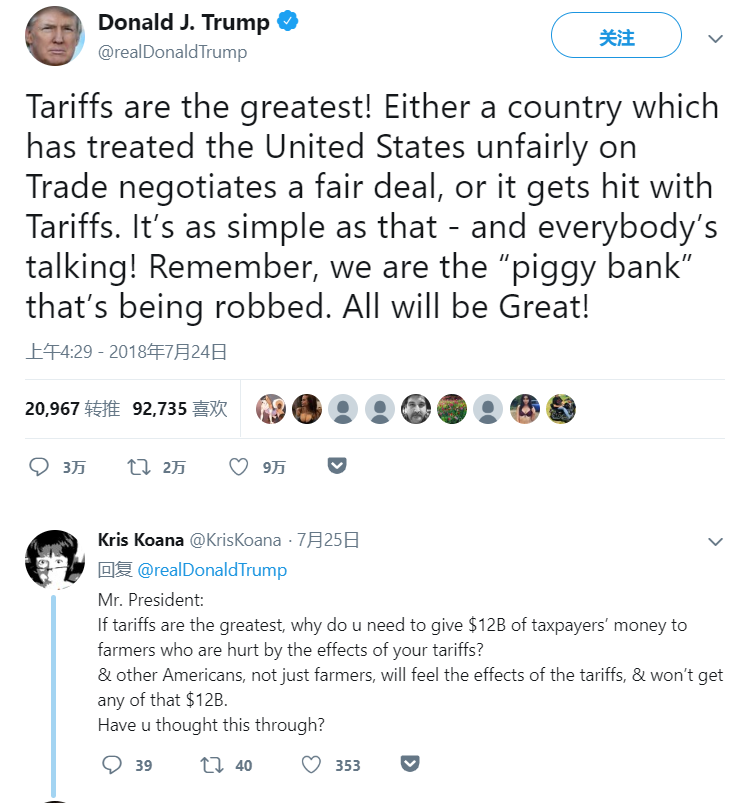
\includegraphics[scale=0.5]{fig/instruments/trump.png}
 	\end{column}
 
  	\begin{column}{0.4\textwidth}
 
 	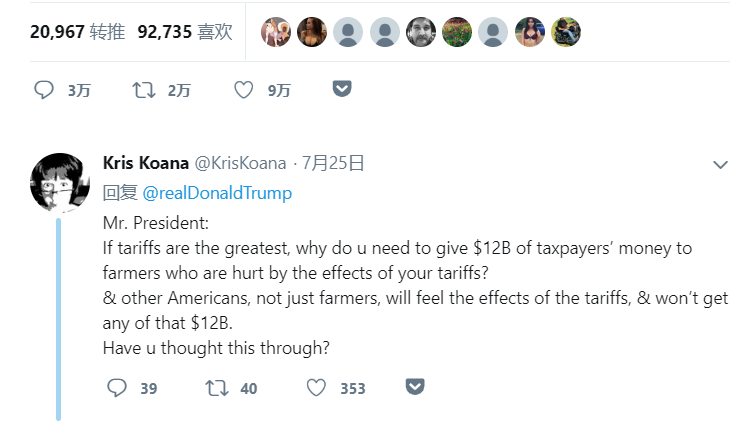
\includegraphics[scale=0.4]{fig/instruments/trump2.png}
 \end{column}
 \end{columns}

\end{frame}

\begin{frame}{Motivating Example}

\begin{itemize}
	\item “Chicken Tax” originally a retaliation by Lyndon Johnson’s administration
	to tariffs imposed on U.S. exports of chicken to Europe (early 1960s) 
	
	\begin{itemize}
		\item Tariff protected European chicken producers but it was defended by
		arguing that hormone use affected male virility 
	\end{itemize}
	\item U.S. retaliated with a 25\% tariff on imports of light commercial
	trucks (still in place 50 years later!) 
	\item Retaliation was focused on Germany (one of the main political proponents
	of the original tariff) and Volkswagen in particular
\end{itemize}
\end{frame}

\begin{frame}{Volkswagen Produced Trucks?}


\begin{figure}


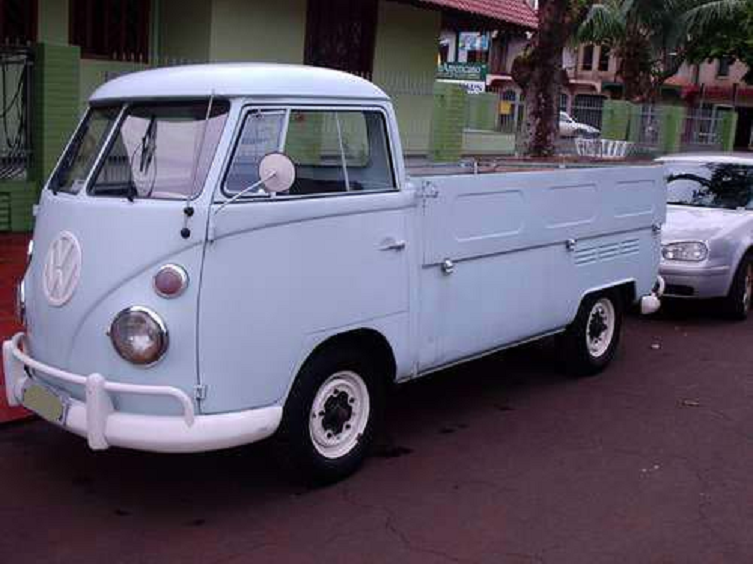
\includegraphics[scale=0.4]{fig/instruments/lec07-1}
\end{figure}

\end{frame}

\begin{frame}{Tariffs Perpetuated}

\begin{itemize}
\item Volkswagen stopped producing light trucks, but by then the “big three”
auto and truck producers were concerned about competition from Japan 
\item Chrysler, Ford, GM successfully lobbied to keep a 25\% tariff 
\item For a while, Subaru’s response to the tariff was to introduce a “passenger”
vehicle (subject to the substantially lower 2.5\% tariff)
\end{itemize}
\end{frame}

\begin{frame}{Meet the Subaru BRAT}


\begin{figure}


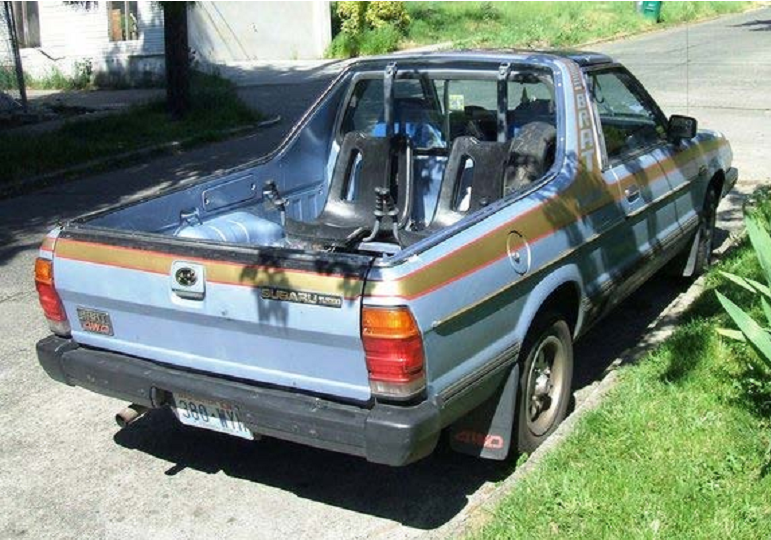
\includegraphics[scale=0.4]{fig/instruments/lec07-2}

\end{figure}

\end{frame}

\begin{frame}{Indirect and Unforeseen Costs}

\begin{itemize}
\item Latest firm to be hit by the tariff is Ford − one of the initial proponents
of the tariff!
\end{itemize}

\begin{columns}[onlytextwidth]
\begin{column}{0.5\textwidth}
\begin{itemize}
\item Ford produces and sells the Ford Transit as a commercial truck in
Europe
\item ... but the “truck” looks quite different when it is shipped to the
U.S., before being reconverted into a truck
\end{itemize}

\end{column}
\begin{column}{0.5\textwidth}
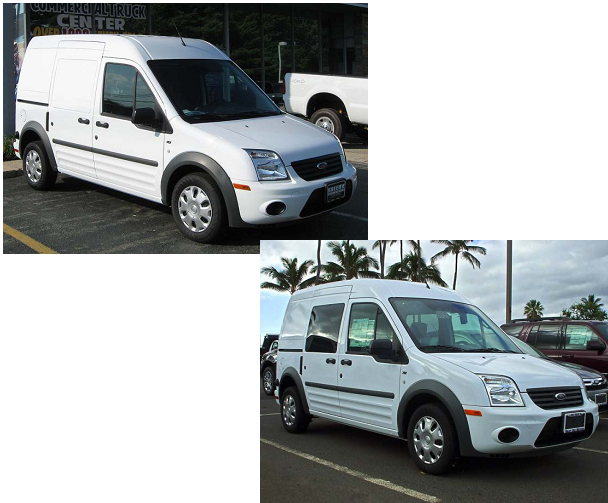
\includegraphics[width=\columnwidth]{fig/instruments/lec07-3}
\end{column}
\end{columns}

\end{frame}



\section{The Instruments of Trade Policy}


\subsection{Types of Protection and analytical tools}
\begin{frame}{Different Types of Protection}

\begin{itemize}
\item The classic instrument of protection is the\textbf{\textcolor{red}{\emph{
tariff}}}, a tax on imports 

\begin{itemize}
\item these can be either specific (a fixed charge per unit) or advalorem
(as a fraction of the value of imported goods) 
\end{itemize}
\item \textbf{\textcolor{red}{\emph{Export subsidies}}} are another form
of protection (e.g., European agricultural goods) 
\item \textbf{\textcolor{red}{\emph{Import quotas}}} are quantity restrictions
(import side) 
\item \textbf{\textcolor{red}{\emph{Voluntary Export Restraints (VERs)}}}
are analogous to import quotas but on the export side 
\item \textbf{\textcolor{red}{\emph{Regulations}}} of various types may
act as protection
\end{itemize}
\end{frame}

\begin{frame}{Types of Tariffs}
 \begin{columns}[onlytextwidth]
 	\begin{column}{0.6\textwidth}
 	 \begin{itemize}
 		\item Classification on the Basis of Criterion for Imposition
 		\begin{itemize}
 			\item Specific Tariffs从量税
 			\item Ad Valorem Tariffs从价税
 			\item Compound Tariffs 复合税
 			\item Sliding scale tariff滑准税
 			\item Tariff Quota关税配额
 		\end{itemize}
 		\item Classification on the Basis of Discrimination
 		\begin{itemize}
 			\item Most-Favored Nation Tariffs MFN最惠国关税
 			\item Preferential Tariffs 歧视性关税
 			\item Bound Tariffs 约束税率
 		\end{itemize}
 	\end{itemize}
 \end{column}	

 	\begin{column}{0.4\textwidth}
		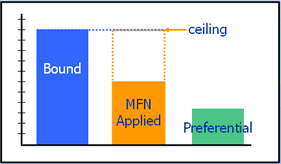
\includegraphics[scale=0.8]{fig/instruments/tariff}
\end{column}
 		
 \end{columns}



\end{frame}

\begin{frame}{Partial Equilibrium Analysis}

\begin{itemize}
\item We next study the effects of an import tariff in \textbf{\textcolor{red}{\emph{partial
equilibrium}}} 
\item By that we mean that we focus on the effects of a tariff on an industry
that is “small” relative to the size of the economy 
\item By “\textbf{\textcolor{red}{\emph{small}}}” we mean that: 

\begin{itemize}
\item No income effects of trade policy feeding back into demand 
\item No effect on wages (or exchange rates) which might feed back into
the supply side 
\item Do not worry about the trade balance being equal to zero 
\end{itemize}
\item Then we can use standard supply and demand analysis
\end{itemize}
\end{frame}

\begin{frame}{Export Supply Function}

\begin{itemize}
\item Denote by $P$ the equilibrium price in the industry under study 
\item Naturally, when $P$ goes up there will be an incentive for

\begin{itemize}
\item domestic producers to expand production 
\item domestic consumers to reduce demand 
\end{itemize}
\item Overall, we have that exports (when positive) will go up 
\item Or, more simply, the export supply function is upward sloping
\end{itemize}
\end{frame}

\begin{frame}{Graphical Derivation of XS出口供给曲线}


\begin{figure}


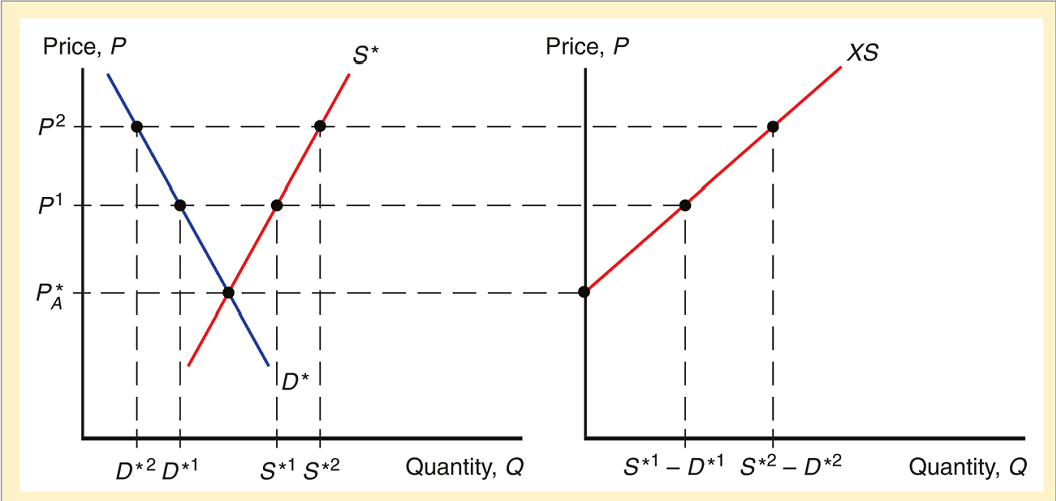
\includegraphics[scale=0.4]{fig/instruments/lec07-4}

\end{figure}

\end{frame}

\begin{frame}{Import Demand Function}

\begin{itemize}
\item What happens when $P$ is lower than $P_{A}^{*}$? 
\item Then the country imports the good 
\item And the lower is $P$, the larger is the volume of imports 
\item Hence, the import demand function is downward sloping
\end{itemize}
\end{frame}

\begin{frame}{Graphical Derivation of MD}


\begin{figure}


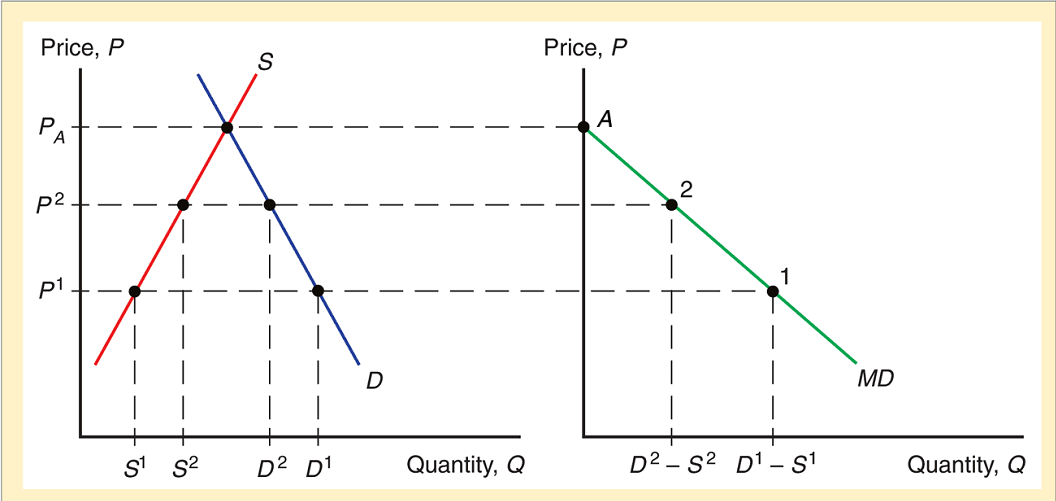
\includegraphics[scale=0.4]{fig/instruments/lec07-5}

\end{figure}

\end{frame}

\begin{frame}{Equilibrium}


\begin{columns}[onlytextwidth]
\begin{column}{0.5\textwidth}
\begin{itemize}
\item the equilibrium will achieve where $MD$ and $XS$ intersect.  
\item Say, domestic import demand equals foreign export supply 
\item This determines the equilibrium world price $P_{W}$
\item $Q_W$ is the amount of export/import
\end{itemize}

\end{column}
\begin{column}{0.5\textwidth}
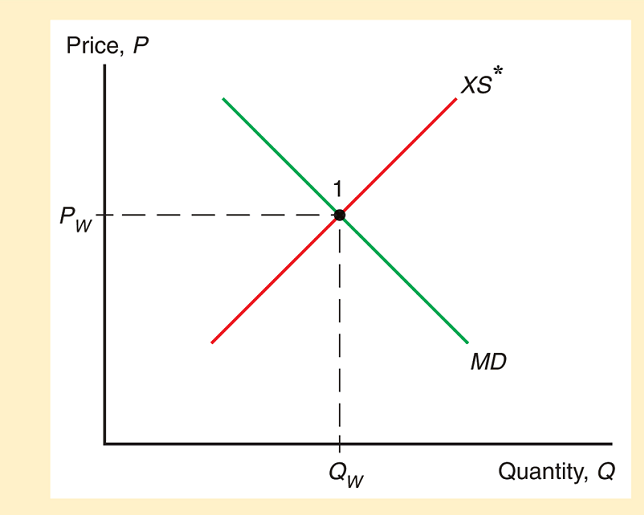
\includegraphics[width=\columnwidth]{fig/instruments/lec07-6}
\end{column}
\end{columns}

\end{frame}



\subsection{Effect of Tariff}
\begin{frame}{Effect of Tariff-大国情形}

\begin{itemize}
	\item 思考:美国对来自中国进口商品征收关税,关税的实际承担者是谁?
\item Now suppose that the Home country levies a specific\textbf{\textcolor{red}{\emph{
tariff}}} \textbf{\textcolor{red}{\emph{$t$}}} on imports from Foreign 
\item Foreign producers will not be able to sell at Home unless the price
difference between the domestic and foreign markets is at least as
large as the tariff 
\item At the original price, there is excess demand in the domestic market
and excess supply in the foreign market 
\item The price will tend to rise in the domestic market, while 
\item it will tend to fall in the foreign market
\end{itemize}
 \begin{block}{总结}
 	引进关税就好比在两国的价格之间插上了一个楔子
 \end{block}

\end{frame}

\begin{frame}{Graphical Analysis}

\begin{itemize}
\item The difference in prices will settle at $P_{T}–P_{T}^{*}=t$,
but the domestic price goes up by less than $t$ (always?)
\begin{figure}


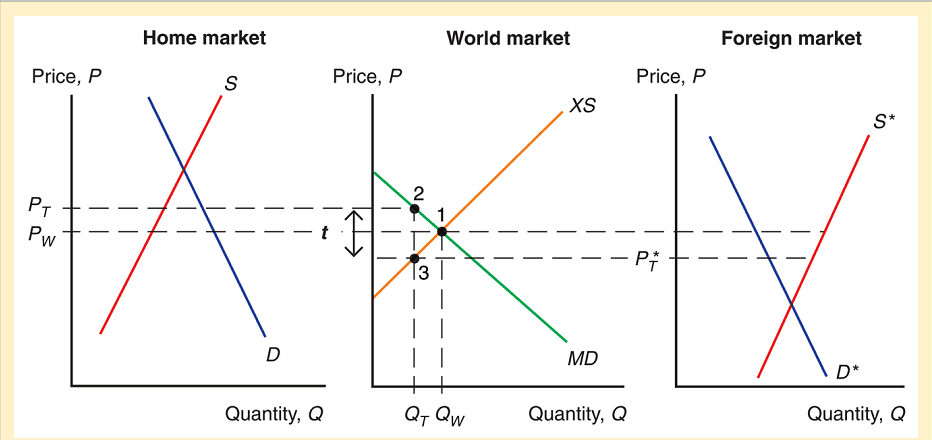
\includegraphics[scale=0.4]{fig/instruments/lec07-7}
\end{figure}

\end{itemize}
\end{frame}

\begin{frame}{Effect of Tariff-小国情形}
 \centering	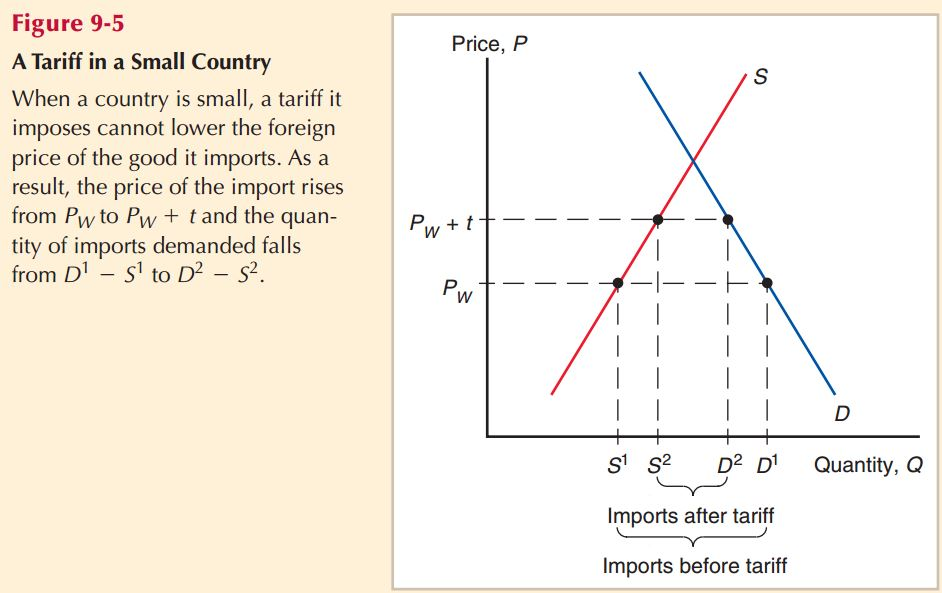
\includegraphics[scale=0.4 ]{fig/instruments/small}
\end{frame}

\begin{frame}{Costs and Benefits of Tariffs——评判标准}

\begin{itemize}
\item An import tariff raises the domestic price so we expect that the tariff
will \textbf{\textcolor{red}{\emph{hurt consumers, but benefit producers}}} 
\item In addition, the government obtains some tariff revenue, which may
be rebated back to consumers (directly or more realistically indirectly) 
\item What is the net effect? 
\item We can study this by appealing to the concepts of consumer surplus
and producer surplus
\end{itemize}
\end{frame}

\begin{frame}{Consumer Surplus}

\begin{block}{Consumer surplus measures the sum of the differences in the prices
actually paid by consumers from the maximum prices they would be willing
to pay for each unit consumed}


\begin{figure}
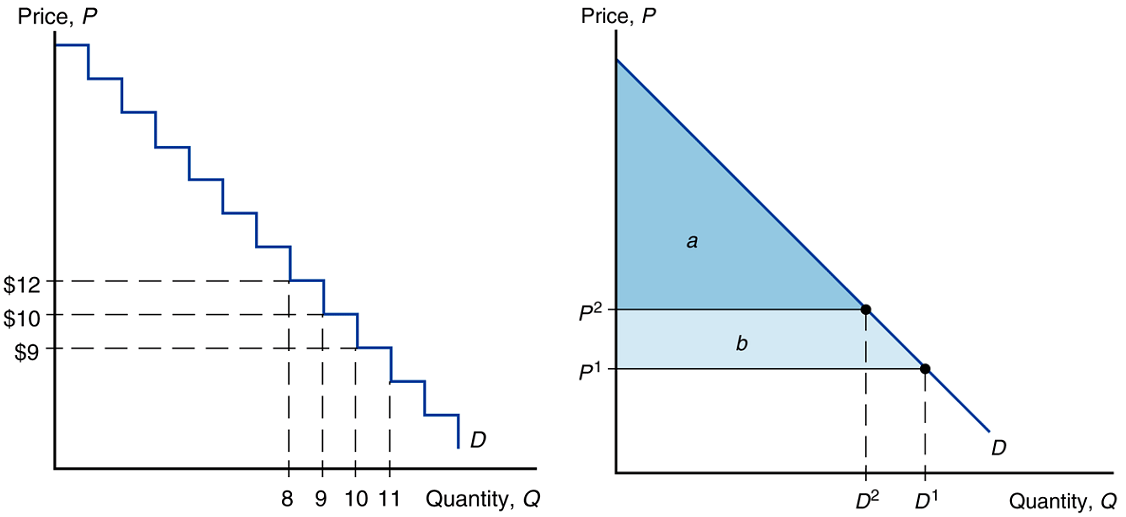
\includegraphics[scale=0.3]{fig/instruments/lec07-8}
\end{figure}



\end{block}
\end{frame}

\begin{frame}{Producer Surplus}

\begin{block}{Producer surplus measures the amount that producers gain from sales
by computing the difference between the price received and the minimum
price at which they would be willing to sell}


\begin{figure}


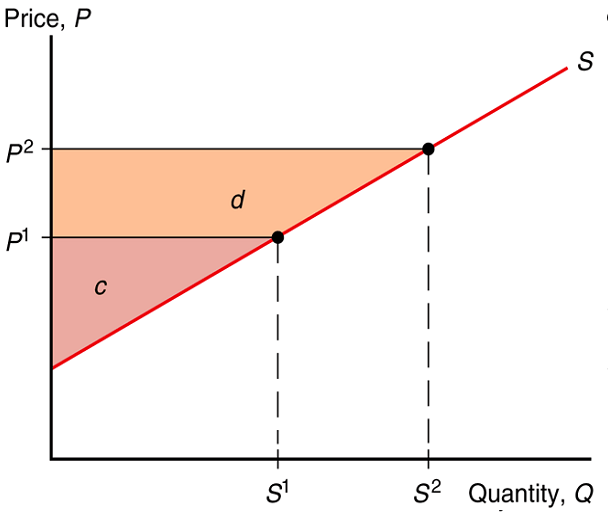
\includegraphics[scale=0.3]{fig/instruments/lec07-9}

\end{figure}

\end{block}
\end{frame}

\begin{frame}{Decomposition of the Effect}


\begin{columns}[onlytextwidth]
\begin{column}{0.5\textwidth}
\begin{itemize}
\item The price increase reduces consumer surplus by an amount $a+b+c+d$
\item But producer surplus increases by $a$ 
\item On top of that, $c+e$ is collected in tariff revenue
\end{itemize}

\end{column}
\begin{column}{0.5\textwidth}
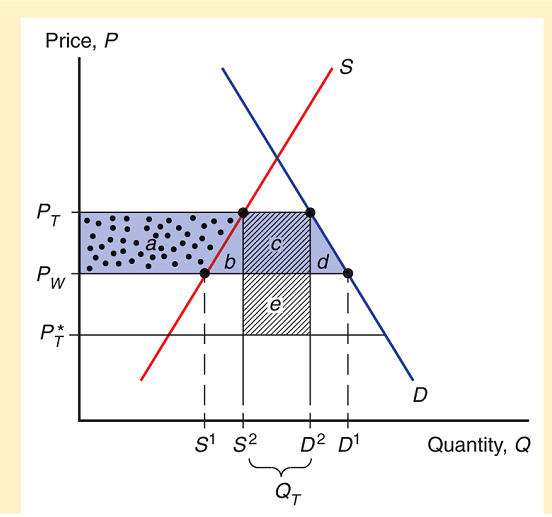
\includegraphics[width=0.9\columnwidth]{fig/instruments/lec07-10}
\end{column}
\end{columns}

\end{frame}

\begin{frame}{Net Effect}

\begin{itemize}
\item Notice that the net effect is in general ambiguous: it is given by
$e-(b+d)$
\item The triangles b and d represent an efficiency loss 

\begin{itemize}
\item tariff distorts production and consumption decisions (too much production,
too little consumption) 
\end{itemize}
\item The rectangle $e$ represents a terms of trade gain 

\begin{itemize}
\item for a large enough country, the tariff will reduce the (untaxed) export
price cashed by foreigners 
\end{itemize}
\item What happens when the country is small?
\end{itemize}
	\pause
	\begin{block}{结论}
		大国征收关税有可能获益,但是小国征收关税必受损
	\end{block}
\end{frame}

\begin{frame}{Effective Rate of Protection有效保护率}

\begin{itemize}
\item Do you think tariffs would be a good measures of the effective rate
of protection,或者说,关税越高,表示保护程度越高

\begin{itemize}
\item Absolutely No (because they tax gross value, not value added )
\end{itemize}
\item Example: suppose that a car sells on the world market for \$8000,
and the parts that made it are worth \$6000 
\item The value added of the car production is \$2000 
\item Suppose that a country puts a 25\% tariff on imported cars and domestic
price goes up to \$10,000 
\item 那么对于汽车产业的保护率是否就是25\%呢?
\item Cost of assembly can be 100\% higher than before!\end{itemize}


\end{frame}

\begin{frame}
\begin{definition}[有效保护率]
The effective rate of protection for a sector is formally defined
as: 

\[
ERP=\frac{V_{T}-V_{W}}{V_{W}}
\]


where $V_{W}$ is value added in the sector at world prices and $V_{T}$
is value added in the presence of trade policies.
\end{definition}
\begin{block}{如果要保护国内的汽车零部件生产,将会对汽车组装业造成怎样的影响}
	\begin{itemize}
		\item imposes a 10 percent tariff on imported parts
		\item raising the cost of parts of domestic	assemblers from \$6,000 to \$6,600
		\item no change in the tariff on assembled automobiles
		
	\end{itemize}
\end{block}

\end{frame}



\subsection{Import Quotas}
\begin{frame}{Import Quotas}

\begin{itemize}
\item Remember that an import tariff tends to reduce the volume of imports
into the domestic market 
\item A \textbf{\textcolor{red}{\emph{more straightforward}}} way to achieve
the same goal is by directly restricting the volume of imports: an
\textbf{\textcolor{red}{\emph{import quota }}}
\item This quota is usually enforced by issuing licenses to domestic importing
firms or to foreign exporting countries’ governments 
\item If the quota is binding, the domestic price will rise because of the
associated excess demand
\end{itemize}
\end{frame}

\begin{frame}{Welfare Effects of Import Quotas}

\begin{itemize}
\item The analysis is essentially identical to that of import tariffs 

\begin{itemize}
\item For each tariff there is a quota that implements the same change in
import volumes and prices 
\end{itemize}
\item But notice that the government is not collecting any tariff revenues
in the quota case 
\item Is a quota always worse? 
\item Only when all quota rents are \textbf{\textcolor{red}{\emph{collected
by domestic agents}}} will the two instruments be equally effective 

\begin{itemize}
\item Example: U.S. Sugar quota rents go to foreign gov’s 
\item Sugar quotas save jobs, but they cost \$826,000 per job
\end{itemize}
\end{itemize}
\end{frame}

\frame{
	\frametitle{US Sugar quota}
	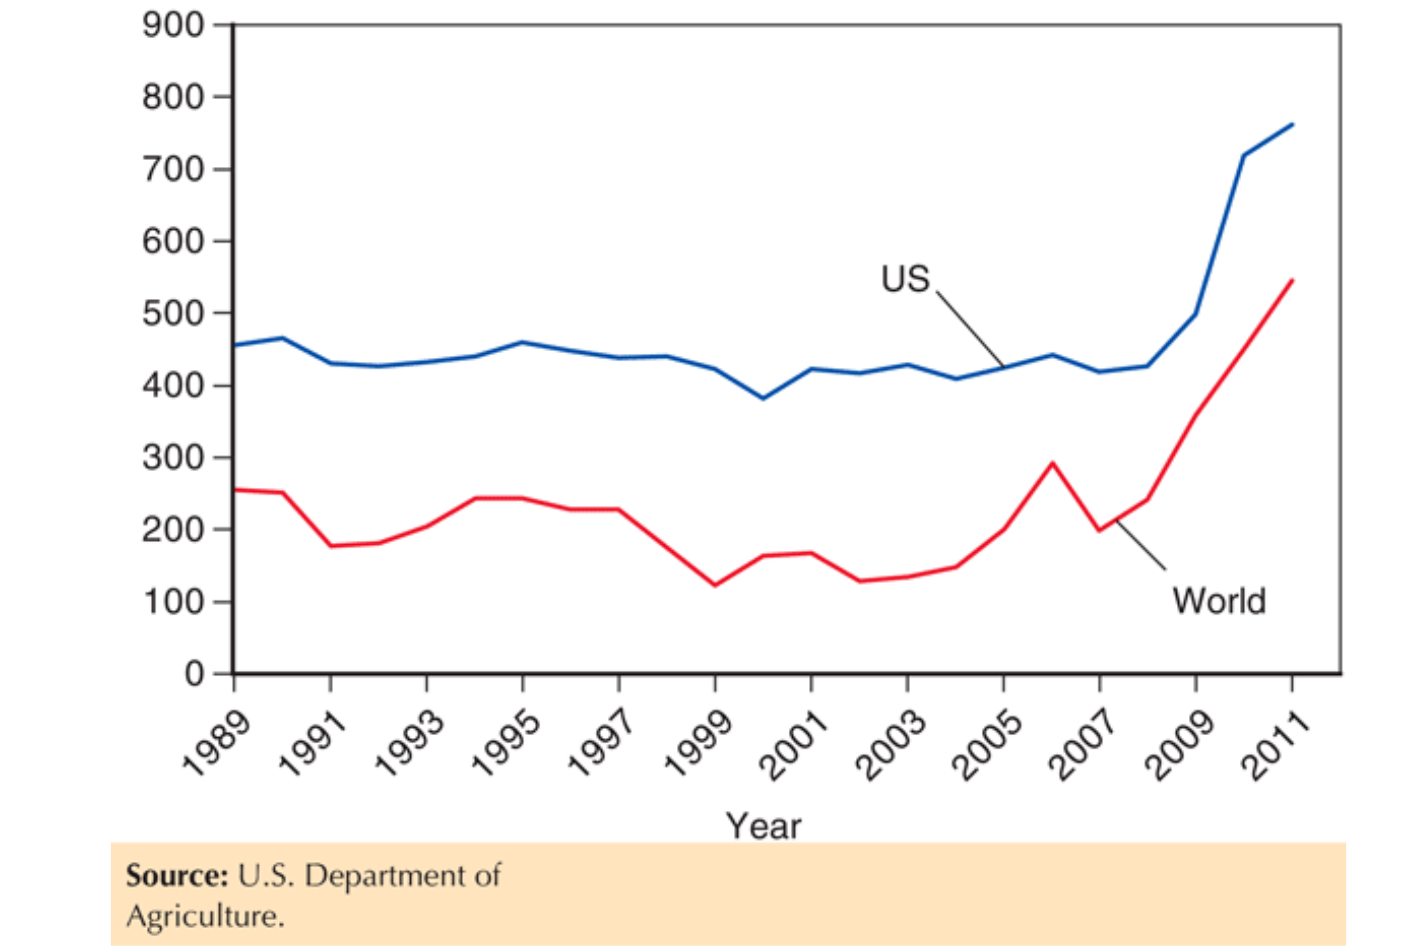
\includegraphics[scale=0.20]{fig/instruments/us_sugar.png}
}

\frame{
	\frametitle{US Sugar quota}
	\begin{itemize}
		\item textbook: \emph{If the sugar restrictions were lifted, the drop in the refined sugar price would induce a substantial expansion in the sugar-using food industry}
		\item Maybe they should keep the quota\dots
	\end{itemize}
	\begin{center}
		
\includegraphics[scale=0.5]{fig/instruments/fat-american.jpg}
	\end{center}
}




\subsection{Export Subsidies}
\begin{frame}{Export Subsidies}

\begin{itemize}
\item \textbf{\textcolor{red}{\emph{Export subsidies}}} were used very widely
(now somewhat less so) by the EU under its CAP(Common Agricultural
Policy) 
\item An export subsidy raises the price of a good in the exporting country,
while lowering it in foreign countries 
\item 出口补贴只有在商品出口时才会获得补贴,为什么会提高国内的价格呢?
\item Consumers are worse off, producers are better off, and government
revenue is negative 
\item The welfare effects are unambiguously negative overall
\item If there is a export subsidies, which market would the producer prefer?
Home or Foreign?
\end{itemize}
\end{frame}

\begin{frame}{Export Subsidies: Welfare Analysis}


\begin{columns}[onlytextwidth]
\begin{column}{0.5\textwidth}
\begin{itemize}
\item Consumer surplus goes down by $a+b$ 
\item Producer surplus goes up by $a+b+c$
\item The required government expenditure is $b+c+d+e+f+g$
\item So net loss is $b+d+e+f+g$

\begin{itemize}
\item of these, $b$ and $d$ are efficiency losses 
\item $e+f+g$ is the terms-of trade loss
\end{itemize}
\end{itemize}

\end{column}
\begin{column}{0.5\textwidth}
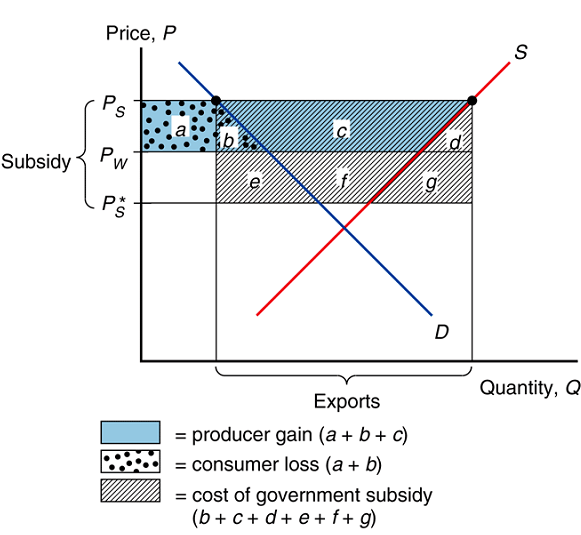
\includegraphics[width=0.9\columnwidth]{fig/instruments/lec07-11}
\end{column}
\end{columns}

\end{frame}

\begin{frame}{European Subsidies}

\begin{itemize}
\item The European Union’s Common Agricultural Policy sets high prices for
agricultural products and subsidizes exports to dispose of excess
production 

\begin{itemize}
\item In fact, without these subsidies, Europe would be a net importer of
most of these agricultural goods 
\end{itemize}
\item The direct cost of this policy for European taxpayers was almost \$76
billion in 2009 

\begin{itemize}
\item There are proposals to make these subsidies independent of production
(preferred policy)
\end{itemize}
\end{itemize}
\end{frame}



\subsection{Other Instruments of Trade}
\begin{frame}{Export Taxes}

\begin{itemize}
\item Using an analogous analysis, one can show that export taxes may be
welfare-enhancing 
\item Oil-producing countries sometimes use export taxes 
\item Or China more recently in the case of rare earth metals (tungsten)15%
\item 2015年4月23日,财政部发布消息称经国务院批准取消稀土、钨、钼、钢铁颗粒粉末等产品的出口关税,自2015年5月1日起实施。
\item 自2015年1月1日开始,中国稀土出口配额制正式取消
\end{itemize}
\end{frame}

\begin{frame}{Voluntary Export Restraints}

\begin{itemize}
\item A \textbf{\textcolor{red}{\emph{voluntary export restraint}}} is analogous
to an import quota, except that the quota is imposed by the exporting
country 
\item These restraints are however usually requested by the importing country 
\item Example: limitation on Japanese exports of autos in 1981 
\item The profits or rents from this policy are earned by foreign governments
or foreign producers 
\item Sometimes VERs are multilateral in nature (ex: MFA)

\begin{itemize}
\item The Multi Fibre Arrangement (MFA) governed the world trade in textiles
and garments from 1974 through 2004, imposing quotas on the amount
developing countries could export to developed countries. It expired
on 1 January 2005.
\end{itemize}
\end{itemize}
\end{frame}

\begin{frame}{Local Content Requirements当地成分要求}

\begin{itemize}
\item A local content requirement is a regulation that requires that some
specified fraction of a final good be produced domestically \
\item TRIMS(与贸易有关的投资措施协议(Trade Related Investment Measures)) 协议的一部分
\item Provides protection for domestic producers of inputs (similar to import
quota) 对国内投入品制造商提供了一定的保护
\item From the viewpoint of firms that must buy domestic inputs, it is a
bit more flexible than an import quota (can expand domestic input
purchases) 
\item Local content requirement provides neither government revenue (as
a tariff would) nor quota rents
\end{itemize}
\end{frame}

\begin{frame}{Other Trade Policy Instruments}

\begin{itemize}
\item Export credit subsidies 

\begin{itemize}
\item A subsidized loan to exporters (Ex: US Export-Import Bank;中国进出口银行) 
\end{itemize}
\item National procurement 政府采购

\begin{itemize}
\item Government agencies are sometimes obligated to purchase from domestic
suppliers (even when they charge higher prices than foreigners) 
\item 以上行为受WTO《政府采购协议》(GPA)约束
\end{itemize}
\item Bureaucratic regulations 行政性法规

\begin{itemize}
\item Safety, health, quality or customs regulations(can act as a form of
protection and trade restriction (Ex: Poitiers 1982)
\end{itemize}
\end{itemize}
\end{frame}

\begin{frame}{summary}
\centering 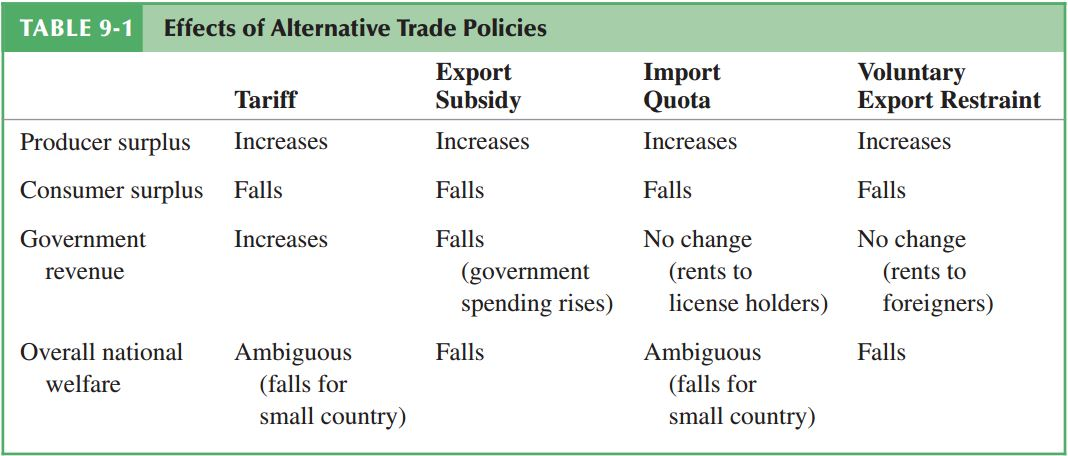
\includegraphics[scale=0.5]{fig/instruments/summary}

\end{frame}





\end{document}
